\documentclass{beamer}
\mode<presentation>
\usepackage[utf8]{inputenc}
\usepackage{graphicx}
\usepackage[english,italian]{babel} % se non fosse inglese dovrei indicare la lingua nella quale sillabare [Italian]
%\usepackage{fancybox}
\useoutertheme{}
\usepackage{beamerthemeshadow}
\usepackage{ulem}
\usepackage{courier}
\usepackage{tikz}
\usepackage{listings}
\usepackage{amsfonts}
\usepackage{fontawesome5}
\usepackage{color,soul}
\usetikzlibrary{snakes}
%\usepackage{beamertexpower}
%\beamertemplatetransparentcovereddynamicmedium
\usetheme{GTER} %(se vuoi mettere l'autore)
\useinnertheme{rectangles}
%\useoutertheme{infolines}
\usecolortheme[RGB={151,215,0}]{structure}
%\usecolortheme[RGB={0,99,29}]{palette quaternary}

\setbeamercovered{transparent}
\setbeamerfont{frametitle}{size=\small,series=\bfseries}
\setbeamercolor{frametitle}{bg=gter!}

\definecolor{lightred}{rgb}{0.94,0.04,0.04}
\definecolor{aqua}{rgb}{0.00,0.80,1.00}
\definecolor{lightgreen}{rgb}{0.01,0.40,0.03}
\definecolor{limegreen}{rgb}{0.61,1.00,0.10}
\definecolor{peach}{rgb}{1.01,0.85,0.72}
\definecolor{purple}{rgb}{0.93,0.51,0.93}
\definecolor{indianyellow}{rgb}{0.98,0.75,0.30}
\definecolor{brick}{rgb}{0.70,0.13,0.13}
\definecolor{springsteen}{rgb}{0.00,0.49,0.19}
%%%%%%%%%%%%%%%%%%%%%%%%%%%%%%%%%%%%%%%%%%%%%%%%%%%%%%%%%%%%%%%%%%%%%%
% \definecolor{gter}{rgb}{0.00,0.49,0.22} %verde GTER estratto da gimp
\definecolor{gter}{RGB}{151,215,0}
%%%%%%%%%%%%%%%%%%%%%%%%%%%%%%%%%%%%%%%%%%%%%%%%%%%%%%%%%%%%%%%%%%%%%%
\definecolor{lightorange}{rgb}{1.01,0.50,0.00}
\definecolor{royalblue}{rgb}{0.25,0.41,1.00}
\definecolor{lightgray}{rgb}{0.94,0.94,0.94}

% \definecolor{links}{HTML}{2A1B81}
\hypersetup{colorlinks,linkcolor=lightgray,urlcolor=springsteen}

\title{Modulo 3 - Georeferenziazione}
\subtitle{Gestione dei formati .dwg, .pdf, .gpx}
\author[]{Gter srl Innovazione in Geomatica Gnss e Gis}
\author[]{Relatore: Simone Parmeggiani}
\date{Genova, Marzo 2024} 
\logo{
\includegraphics[height=0.5 cm]{./Gter.png}}

\begin{document}
	{
		{
			\setbeamertemplate{footline}{} 
			\begin{frame}
				\titlepage
			\end{frame}
		}
		\addtocounter{framenumber}{-1}

\section{File .dwg}
\subsection{Metodo 1}

\begin{frame}
   \frametitle{Metodo 1: creazione dxf}

   Il formato .dwg è un formato proprietario e non viene letto direttamente da QGIS come avviene per molti altri formati. Infatti, facendo il classico Drag and Drop otteniamo un messaggio di errore:

    \begin{figure}[h]
        \centering
        
\includegraphics[width=1.2\textwidth]{pics/drag_n_drop.png}
    \end{figure}   

    \textbf{Invalid Data Source: *percordo del file* is not a valid or recognized data source.}
    
     
\end{frame}

\begin{frame}
   \frametitle{Metodo 1: creazione .dxf}

   Pertanto è necessario passare attraverso un formato vettoriale di interscambio: il .dxf
   Dal software CAD utilizzato per generare il .dwg scegliere "salva come" ed esportare il progetto in \textbf{AutoCAD 200 ASCII DXF}.

    A questo punto sarà possibile fare un drag and drop, che ci porterà ad una finestra di scela su quali layer del file si vuole importare.

\end{frame}

\begin{frame}
   \frametitle{Metodo 1: creazione .dxf}

     Tuttavia, con questo metodo non è possibile visualizzare i layer del .dwg nella TOC di QGIS (si vede un unico layer che contiene tutti quanti i layer del .dxf).
    Per ovviare a questo problema è necessario creare dei file .dxf distinti per ognuno dei layer che si vuole visualizzare distintamente in QGIS (dal programma cad, copiare e incollare \textbf{SULLE COORDINATE ORIGINALI} il layer che si vuole esportare, e successivamente esportartlo come singolo .dxf)
\end{frame}


\begin{frame}
  \frametitle{Metodo 2: creazione .gpkg}
  \begin{columns}
		\begin{column} {0.75\textwidth}	
			Da QGIS è possibile importare direttamente layer da un .dwg, tuttavia è meglio ripulire il file cad da alcuni elementi prima dell'importazione: 
        \begin{itemize}
   		\item block reference,
   		\item spline (convertire in polilinea),
   		\item hatch.
   	\end{itemize}
  		A questo punto possiamo procedere al caricamento seguendo il percorso 				
		\end{column}
		\begin{column} {0.25\textwidth}	
			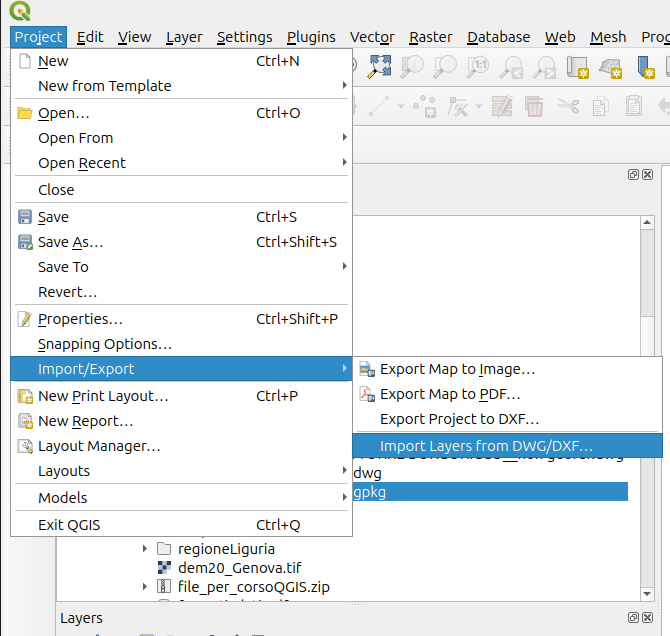
\includegraphics[width=1\textwidth] {./pics/project.png}	
		\end{column}
	\end{columns}
   
  \begin{center}
  		\textbf{Project} $\rightarrow$ \textbf{Import/Export} $\rightarrow$ \textbf{Import Layers from DWG/DXF.}
  \end{center}    
\end{frame} 

\begin{frame}
  \frametitle{Metodo 2: creazione .gpkg}

    \begin{figure}[h]
        \centering
        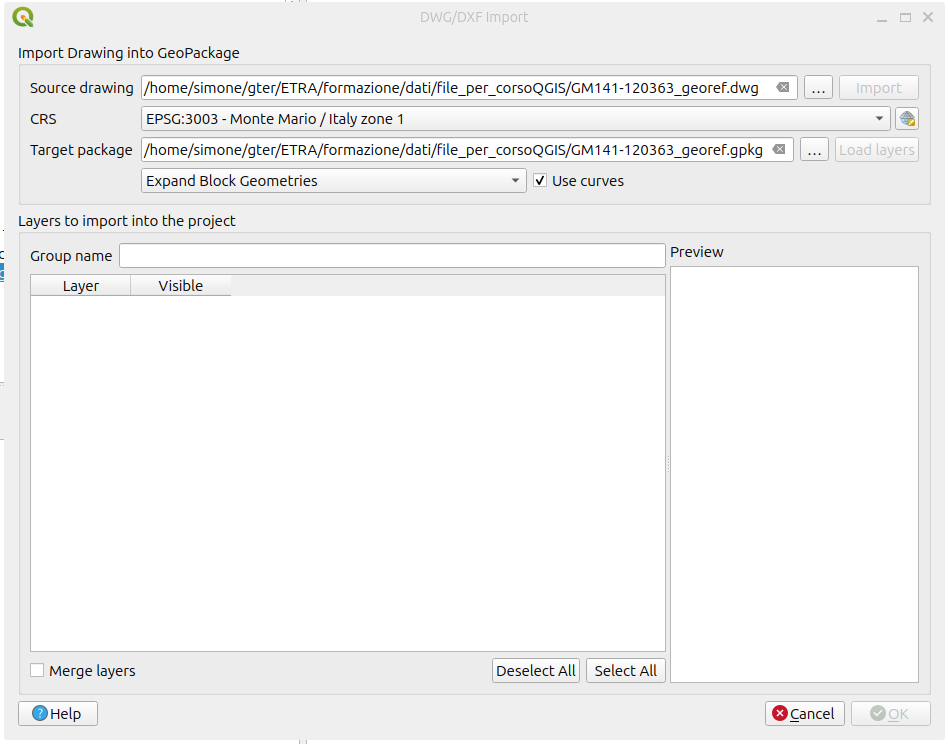
\includegraphics[width=0.7\textwidth]{pics/geopackage.png} 
    \end{figure}
    

\end{frame}

\begin{frame}
  \frametitle{Metodo 2: creazione .gpkg}

    \begin{figure}[h]
        \centering
        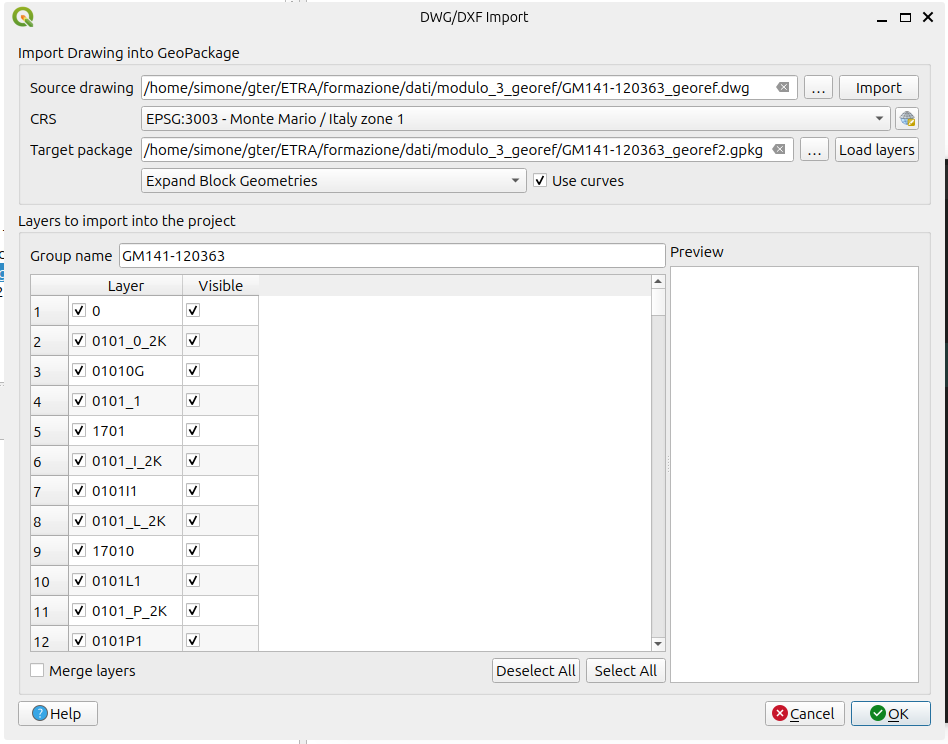
\includegraphics[width=0.7\textwidth]{pics/geopackage2.png} 
    \end{figure}
    

\end{frame} 


\begin{frame}
  \frametitle{Metodo 3: Plugin}
   Infine, è disponibile un plugin di QGIS chiamato \textbf{AnotherDXFImporter} installabile dalla versione 3.0 in poi.
   facendo click su \textbf{Vettore} $\rightarrow$ \textbf{DXF Import / Convert} poi si aprirà l'interfacccia del convertitore che permette di salvare un file .dxf in shapefile o geopackage (Da Testare).
		    
\end{frame}

\begin{frame}
  \frametitle{Metodo 3: Plugin}
   
   \begin{figure}[h]
        \centering
        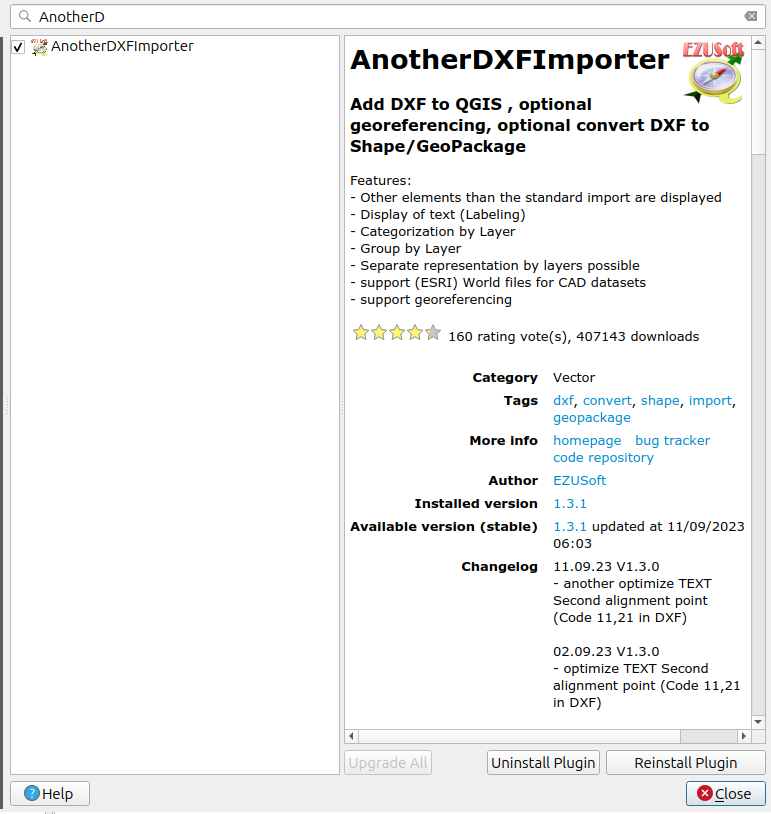
\includegraphics[width=0.6\textwidth]{pics/importer.png} 
    \end{figure}
    
\end{frame} 


\section{Georeferenziazione}

\begin{frame}
    \frametitle{Georeferenziazione}
    Tecnica di attribuzione di coordinate geografiche a un oggetto grafico, usata nelle procedure di cartografia computerizzata e nella costruzione di basi cartografiche digitali.
\end{frame}

 \begin{frame}
   \frametitle{Georeferenziazione}
    \textbf{Layer} $\rightarrow$  \textbf{Georeferenziatore}
    e nella nuova finestra fare clic su  \textbf{File} $\rightarrow$ \textbf{Apri Raster} e caricare il file dell'immagine da georeferenziare.

    L’approccio di base per la georeferenziazione di un raster consiste nel localizzare punti (detti punti fiduciari) sul raster per i quali puoi determinare accuratamente le coordinate.
	   
\end{frame} 

\begin{frame}
    \frametitle{Georeferenziazione}

    \begin{itemize}
        \item Alcune volte nei raster sono presenti punti con le coordinate scritte sull’immagine. In questo caso puoi inserire manualmente le coordinate.
    
        \item Usando layer già georeferenziati. Può trattarsi di dati vettoriali o raster che contengono gli stessi oggetti/geometrie presenti nell’immagine che si desidera georeferenziare e con la proiezione che vuoi per la tua immagine. In questo caso, puoi inserire le coordinate facendo click sul dataset di riferimento caricato nell’area della mappa QGIS.
    \end{itemize}

    
\end{frame} 


\begin{frame}
   \frametitle{Georeferenziazione}
 	\begin{columns}
		\begin{column} {1\textwidth}	
			 \begin{center}
			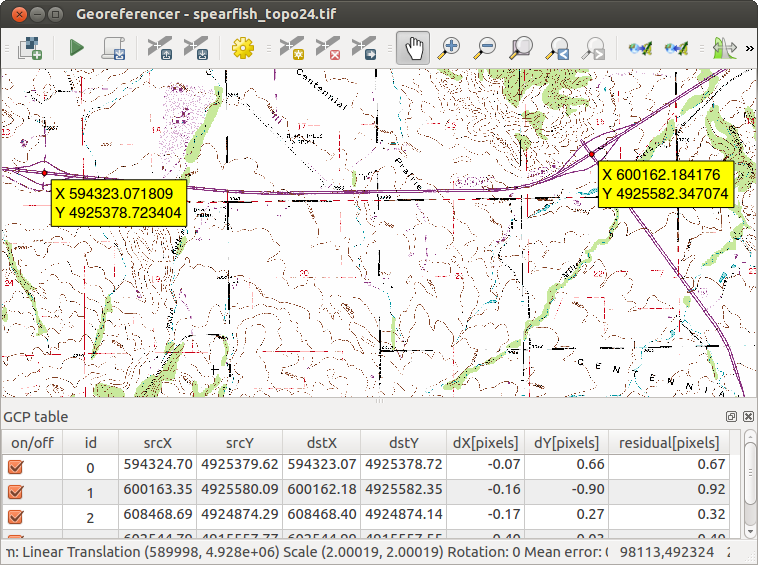
\includegraphics[width=0.8\textwidth] {pics/georef1.png}
		    \end{center}
		\end{column}
 		
	\end{columns}	
	   
\end{frame}

\begin{frame}
\frametitle{Creazione di nuovo layer vettoriale}
    \begin{itemize}
        \item utilizzando il pulsante \textbf{aggiungere un nuovo punto}, si aggiungono punti all’area di lavoro principale e si inseriscono le coordinate (manualmente oppure scegliendolo da un punto della mappa)
    		
        \item Per effettuare una georeferenziazione corretta, è necessario avere almeno 4 punti. Maggiori saranno i punti inseriti, migliore sarà il processo di georeferenziazione (che in ogni caso comporta delle distorsioni, è inevitabile)

        \item E' infine possibile spostare o cancellare un punto inserito
      
    \end{itemize}		
\end{frame} 

\begin{frame}
   \frametitle{file GCP - Ground Control Points}

    I punti che vengono aggiunti alla mappa saranno memorizzati in un file di testo separato (chiamato [nome del file].points) di solito insieme all’immagine raster. Questo ci permette di riaprire il Georeferenziatore in un secondo momento e aggiungere nuovi punti o cancellare quelli esistenti per ottimizzare il risultato. Il file dei punti contiene valori della forma: mapX, mapY, pixelX, pixelY. Puoi usare i pulsanti \textbf{loadGCPpoints - Carica punti GCP e saveGCPPointsAs - Salva punti GCP come } per gestire questi file.
    
\end{frame}

\section{GPS}

\begin{frame}

Il GPS (Global Positioning System) è un sistema di navigazione satellitare di proprietà del governo degli Stati Uniti che, attualmente, comprende 24 satelliti operativi. Il GPS funziona con qualsiasi condizione meteorologica, ovunque nel mondo, 24 ore su 24 e non prevede tariffe di abbonamento o costi di configurazione. Il Dipartimento della Difesa degli Stati Uniti (U.S. Department of Defense, USDOD) ha inizialmente mandato i satelliti in orbita per scopi militari, ma negli anni '80 questi sono stati resi disponibili per l'uso civile.

\end{frame}

\begin{frame}

I file GPS di solito sono salvati in formato .gpx o GPS eXchange Format: è uno schema XML progettato per il trasferimento di dati GPS tra applicazioni software. Può essere usato per descrivere waypoint, tracce e percorsi. I suoi tag contengono queste tipologie di informazioni: location, elevation, e time.

\end{frame}

\begin{frame}

i file .gpx sono importabili in QGIS direttamente con un drag and drop, dopodichè è possibile trattarli come normali file vettoriali.

NB: Un file .gpx deve essere georeferenziato PER DEFINIZIONE in sistema WGS84, essendo un rilievo globale

\end{frame}


\section{Conclusione}

\subsection{Contatti e licenze}
{
\setbeamertemplate{footline}{} 
\setbeamertemplate{headine}{} 
\frame{	
\addtocounter{framenumber}{-1}  % non conto questa slide
\begin{center}
\bigskip

\includegraphics[width=0.2\textwidth]{./Gter.png} \\ 
\scriptsize{
%Gter srl Innovazione in Geomatica Gnss e Gis\\

Via Jacopo Ruffini 9/1A\\
16128, Genova \\
formazione@gter.it\\}
\normalsize
\bigskip
\href{www.gter.it}{\textcolor{gter}{\emph{www.gter.it}}}
	
\bigskip	

  	\href{https://twitter.com/@gteronline} { 
\includegraphics[width=0.15\textwidth]{./tw.jpg}}
	\hspace{30pt}
	 \href{http://www.facebook.com/Gteronline} { 
\includegraphics[width=0.15\textwidth]{./fb.jpg}}
		\hspace{30pt}
%	 \href{ https://plus.google.com/+GterIt/posts} { \includegraphics[width=0.15\textwidth]{../go.png}}
%	 \hspace{30pt}
	 \href{http://www.linkedin.com/company/gter-srl-innovazione-in-geomatica-gnss-e-gis} { 
\includegraphics[width=0.15\textwidth]{./ln.png}}
	 
	 
	 

	 
\bigskip
\vspace{30pt}

	
	\href{http://creativecommons.org/licenses/by-sa/3.0/deed.it} {	
	
\includegraphics[width=0.15\textwidth]{./88x31.png} 
	\\	
	\tiny Quest' opera è distribuita con licenza Creative Commons Attribuzione - Condividi allo stesso modo 3.0 Unported.} 	
	
	
	
\end{center}
%\tableofcontents[pausesections,part=2]
}
}

\end{document}
